\documentclass{beamer}
\usepackage[utf8]{inputenc}

\usepackage{graphicx}

\usetheme{Boadilla}

\title[SybilGuard]{SybilGuard:\\ Defending Against Sybil Attacks via Social Networks}
\author[Dagand, Jezequel]{H. {\sc Yu} \and M. {\sc Kaminsky} \and P. {\sc Gibbons} \and A. {\sc Flaxman}\\
                          Pierre-Evariste {\sc Dagand} \and Loïg {\sc Jezequel}}
\date{January $14^{\mbox{th}}$, 2009}
\institute[PAP]{Pair-à-Pair}

\begin{document}

%%%%%%%%%%%%%%%%%%%%%%%%%%%%%%%%%%%%%%%%%%%%%%%%%%%%%%%%%%%%%%%%

\begin{frame}
\maketitle
\end{frame}

%%%%%%%%%%%%%%%%%%%%%%%%%%%%%%%%%%%%%%%%%%%%%%%%%%%%%%%%%%%%%%%%

\begin{frame}

  \frametitle{Introduction}

  \begin{block}{Sybil Attacks}
    \begin{description}
      \item[Definition:] A malicious user endorses multiple identities  %% Improve this definition ?
      \item[Impact:] Most distributed systems expect a majority of honest users\\
	             Eg.: 2/3 for Byzantine Consensus
    \end{description}
  \end{block}

  \begin{block}{Theoretical Result}
    \begin{description}
      \item[(Douceur02):] ``Thou cannot pass out Sybil nodes in a distributed manner'' %% Find the exact quote...
      \item[Consequence:] Rely on a Central Authority? 
    \end{description}
  \end{block}

\end{frame}

%%%%%%%%%%%%%%%%%%%%%%%%%%%%%%%%%%%%%%%%%%%%%%%%%%%%%%%%%%%%%%%%

\begin{frame}

  \frametitle{SybilGuard}

  \begin{block}{Offering Weaker Guarantees}

    \begin{columns}

      \begin{column}{7cm}
	\begin{itemize}
	\item Bound the number of Sybil nodes
	\item Bound the number of Sybil groups
	\item Accept honest nodes
	\end{itemize}
      \end{column}

      \begin{column}{4cm}
	\vfill
	{\it With High-Probability!}
	\vfill
      \end{column}

    \end{columns}

  \end{block}

  \begin{block}{Benefits}

    \begin{itemize}
      \item Fully decentralized
      \item Handle network dynamics
      \item Leverage Social Networks
    \end{itemize}

  \end{block}

\end{frame}

%%%%%%%%%%%%%%%%%%%%%%%%%%%%%%%%%%%%%%%%%%%%%%%%%%%%%%%%%%%%%%%%

\begin{frame}

  \frametitle{Social Network}
  
  \begin{figure}
    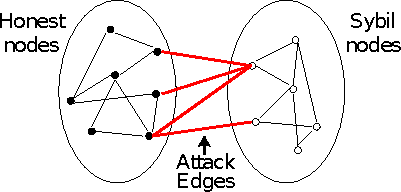
\includegraphics[width=7cm]{./pictures/social_network} \\
    \caption{Social Network}
  \end{figure}

  \begin{block}{Properties}

    \begin{itemize}
    \item Build upon strong trust relationships
    \item \emph{Attack edge}: small quotient cut
    \item Widely studied model
    \end{itemize}

  \end{block}

\end{frame}

%%%%%%%%%%%%%%%%%%%%%%%%%%%%%%%%%%%%%%%%%%%%%%%%%%%%%%%%%%%%%%%%

\begin{frame}

  \frametitle{Random Routes}

  \begin{figure}
    \begin{columns}
      \begin{column}{4.5cm}
	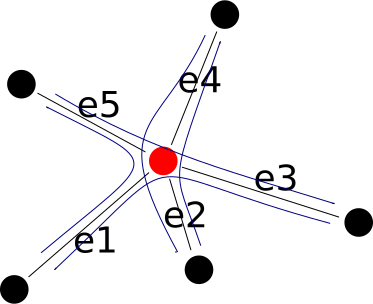
\includegraphics[width=4.5cm]{./pictures/random_route} 
      \end{column}
      \begin{column}{3cm}
	\begin{center}
	  \begin{tabular}{|c|c|c|c|c|}
	    \hline
	    $e_1$ & $e_2$ & $e_3$ & $e_4$ & $e_5$ \\
	    \hline
	    $e_5$ & $e_4$ & $e_1$ & $e_2$ & $e_3$ \\
	    \hline
	  \end{tabular}
	\end{center}
      \end{column}
    \end{columns}

    \caption{Random Routes}
  \end{figure}

  \begin{block}{Properties}
    \begin{description}
      \item[Convergence:] {\small \emph{Two random routes entering an honest node along the same edge will always exit along the same edge}}
      \item[Back-traceability:] {\small \emph{The outgoing edge uniquely determines the incoming edge}}
    \end{description}
  \end{block}

\end{frame}

%%%%%%%%%%%%%%%%%%%%%%%%%%%%%%%%%%%%%%%%%%%%%%%%%%%%%%%%%%%%%%%%

\begin{frame}

  \frametitle{Accepting an honest node}

  \begin{figure}
    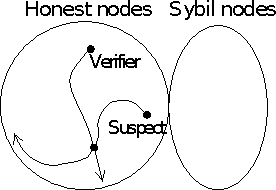
\includegraphics[width=7cm]{./pictures/verify_honest} 
    \caption{Verifying an Honest node}
  \end{figure}

\end{frame}

%%%%%%%%%%%%%%%%%%%%%%%%%%%%%%%%%%%%%%%%%%%%%%%%%%%%%%%%%%%%%%%%

\begin{frame}

  \frametitle{Bounding the number of Sybil groups}

  \begin{figure}
    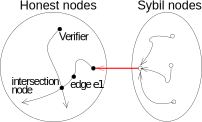
\includegraphics[width=5.5cm]{./pictures/bound_group} 
    \caption{Bounding the number of Sybil groups}
  \end{figure}

  \begin{block}{Case: Single Attack Edge}
    \begin{itemize}
    \item[] All Sybil nodes \emph{have} to go through $e_1$
    \item[$\Rightarrow$] All their routes \emph{have} to intersect the same node %% Convergence
    \item[$\Rightarrow$] Same group (from Verifier's point of view)
    \end{itemize}
  \end{block}

\end{frame}

%%%%%%%%%%%%%%%%%%%%%%%%%%%%%%%%%%%%%%%%%%%%%%%%%%%%%%%%%%%%%%%%

\begin{frame}

  \frametitle{Bounding the number of Sybil nodes}

  \begin{figure}
    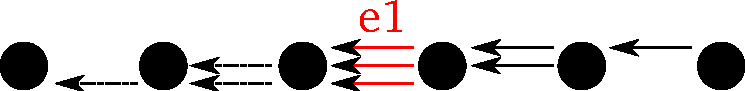
\includegraphics[width=8cm]{./pictures/bound_nodes} 
    \caption{Routes of length 3 sharing an edge}
  \end{figure}
  
  \begin{block}{For an Attack Edge $e_1$}
    \begin{itemize}
      \item[] All Sybil nodes \emph{have} to go through $e_1$
      \item[$\Rightarrow$] At most $w$ routes before the intersection node %% Back-traceability
      \item[$\Rightarrow$] At most $w$ Sybil nodes by Group
    \end{itemize}
  \end{block}

\end{frame}

%%%%%%%%%%%%%%%%%%%%%%%%%%%%%%%%%%%%%%%%%%%%%%%%%%%%%%%%%%%%%%%%

\begin{frame}

  \frametitle{SybilGuard Implementation}

  \begin{block}{Witness Table}
    \begin{itemize}
    \item Details about the $d \times w$ nodes in \emph{downward} routes
    \item To compute intersection nodes
    \item Contain an IP address and a shared secret
    \end{itemize}
  \end{block}

  \begin{block}{Register Table}
    \begin{itemize}
    \item Details about the $d \times w$ nodes in \emph{upward} routes
    \item To verify the source of a routen
    \item Contain a shared secret
    \end{itemize}
  \end{block}

\end{frame}

%%%%%%%%%%%%%%%%%%%%%%%%%%%%%%%%%%%%%%%%%%%%%%%%%%%%%%%%%%%%%%%%

\begin{frame}

  \frametitle{Witness Table}

  \begin{figure}
    \begin{columns}
      \begin{column}{5cm}
	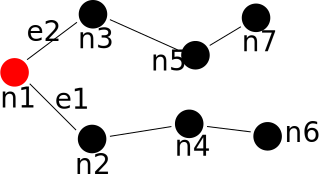
\includegraphics[width=5cm]{./pictures/witness_table} 
      \end{column}
      \begin{column}{5cm}
	\begin{center}
	\begin{tabular}{|c|c|c|}
	  \hline
	  Edge     &  Depth     &  Info \\
	  \hline
	  \hline
	  $e_1$    &  1         &  $(n_2, k_2)$ \\
	  %\hline
	           &  2         &  $(n_4, k_4)$ \\
	  %\hline
	           &  \ldots    &  \ldots       \\
	  \hline
	  \hline
	  $e_2$    &  1         &  $(n_3, k_3)$ \\
	  %\hline
	           & \ldots     &  \ldots       \\
	  \hline
	\end{tabular}
	\end{center}
      \end{column}
    \end{columns}
    \caption{Witness table}
  \end{figure}

  \begin{block}{Scalability}
    \begin{description}
    \item[Space usage:] $O( |k| \times d \times w )$ (real life: 2.56MB)
    \item[Bootstrap:] By propagation along the routes
    \item[Maintainance:] Lazily, with IP address changes
    \end{description}
  \end{block}

\end{frame}

%%%%%%%%%%%%%%%%%%%%%%%%%%%%%%%%%%%%%%%%%%%%%%%%%%%%%%%%%%%%%%%%

\begin{frame}

  \frametitle{Register Table}

  \begin{figure}
    \begin{columns}
      \begin{column}{5cm}
	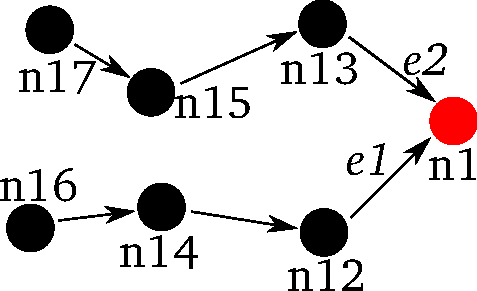
\includegraphics[width=5cm]{./pictures/register_table} 
      \end{column}
      \begin{column}{5cm}
	\begin{center}
	  \begin{tabular}{|c|c|c|}
	    \hline
	    Edge     &  Hop     &  Info \\
	    \hline
	    \hline
	    $e_1$    &  1         &  $k_{12}$ \\
	    %\hline
	    &  2         &  $k_{14}$ \\
	    %\hline
	    &  \ldots    &  \ldots       \\
	    \hline
	    \hline
	    $e_2$    &  1         &  $k_{13}$ \\
	    %\hline
	    & \ldots     &  \ldots       \\
	    \hline
	\end{tabular}
	\end{center}
      \end{column}
    \end{columns}
    \caption{Witness table}
  \end{figure}

  \begin{block}{Scalability}
    \begin{description}
    \item[Space usage:] $O( |k| \times d \times w )$
    \item[Bootstrap:] By propagation along the routes
    \item[Maintainance:] Upon social changes (rare)
    \end{description}
  \end{block}

\end{frame}

%%%%%%%%%%%%%%%%%%%%%%%%%%%%%%%%%%%%%%%%%%%%%%%%%%%%%%%%%%%%%%%%

\end{document}
